\begin{figure}
	\centering
	\subfigure[Impacto zoom: all]{
	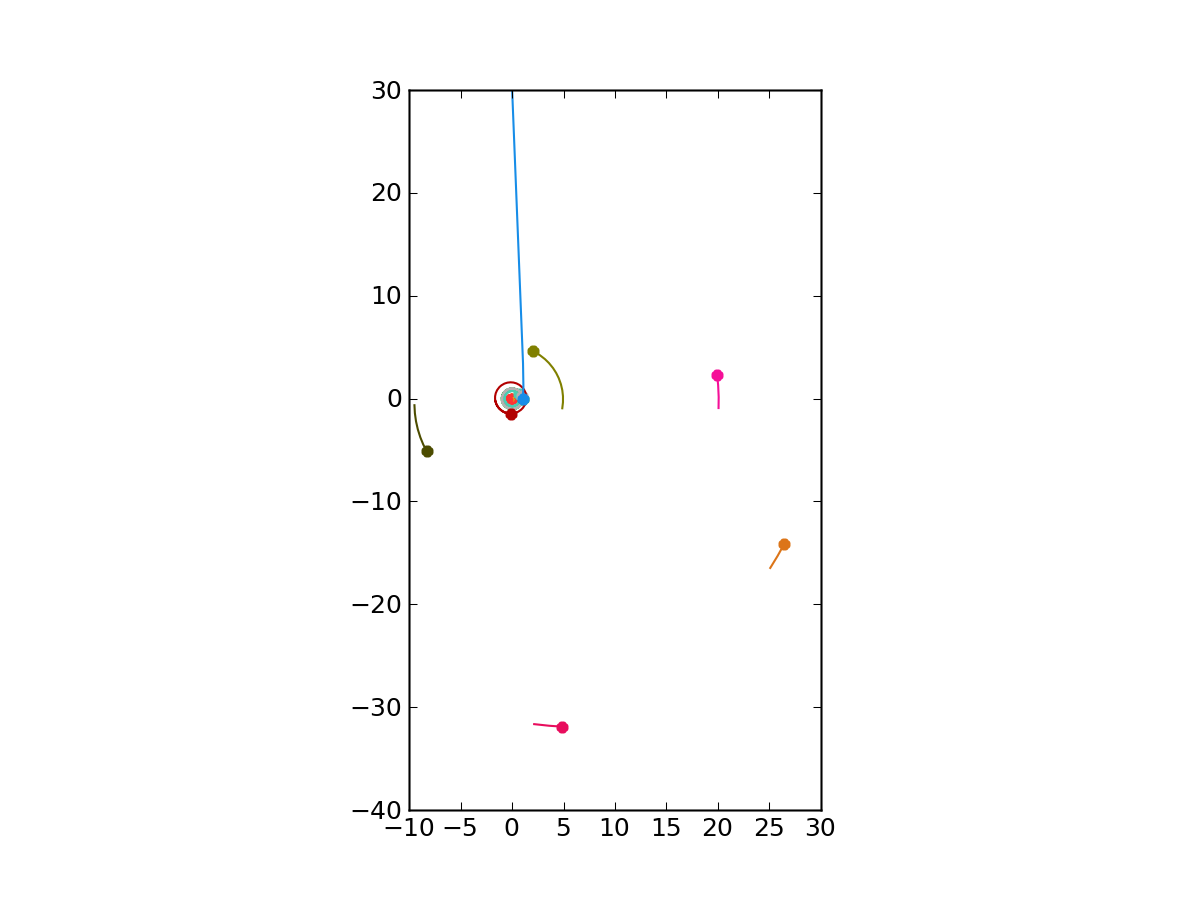
\includegraphics[scale=0.38]{img/bomba/bombaoscurahit_all.png}
	\label{fig:res_bomba_1}
	}
	\subfigure[Impacto zoom: 2.2]{
	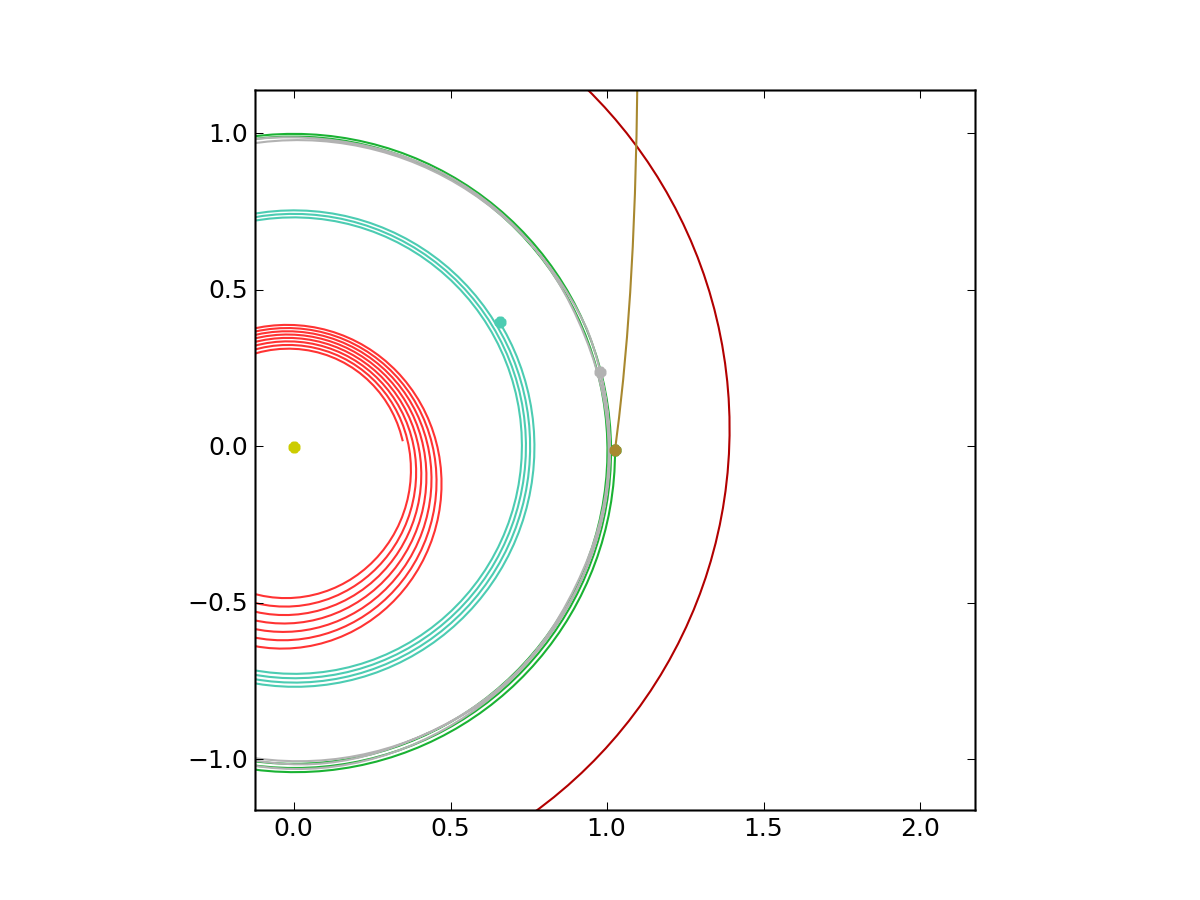
\includegraphics[scale=0.38]{img/bomba/bombaoscurahit_zoom1.png}
	\label{fig:res_bomba_2}
	}
	\\
	\subfigure[Impacto zoom: .2]{
	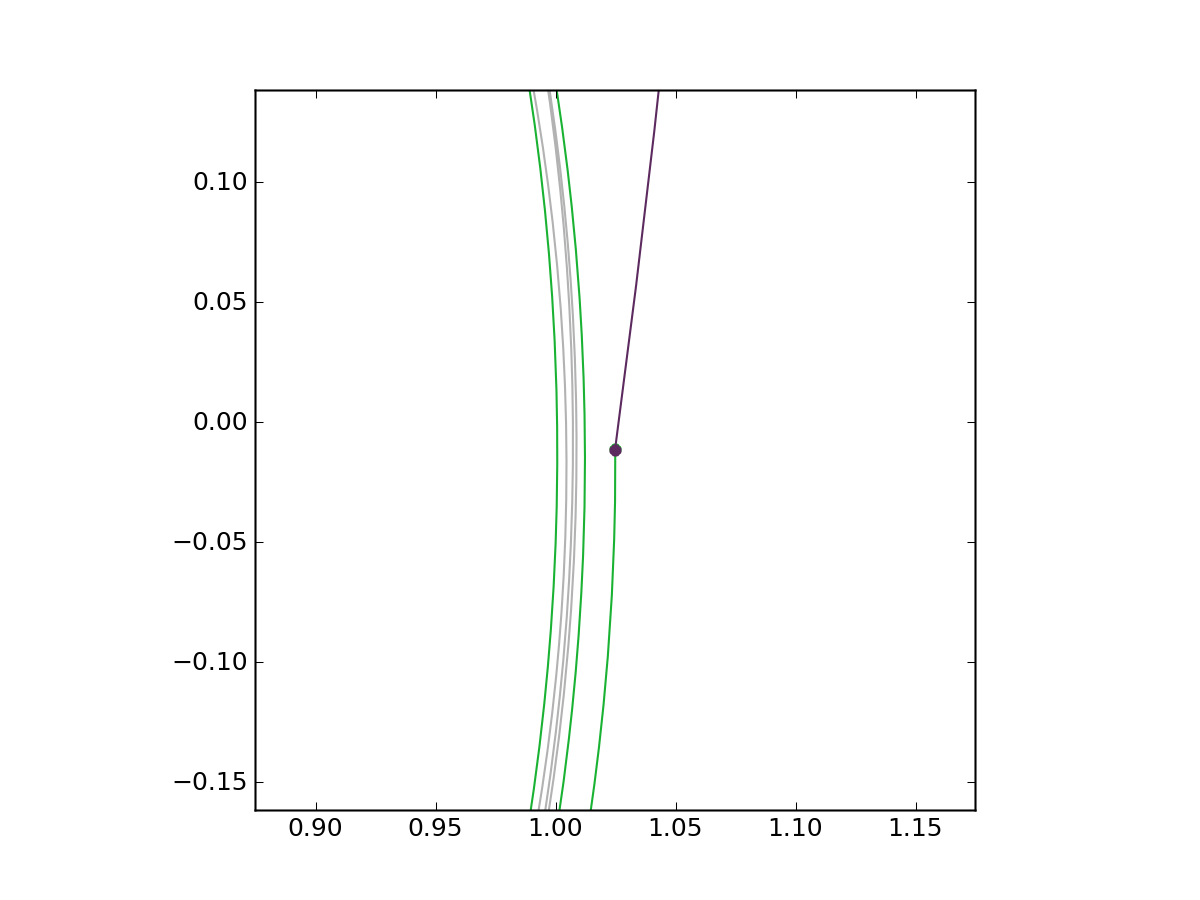
\includegraphics[scale=0.38]{img/bomba/bombaoscurahit_zoom2.png}
	\label{fig:res_bomba_3}
	}
	\subfigure[intento de impacto]{
	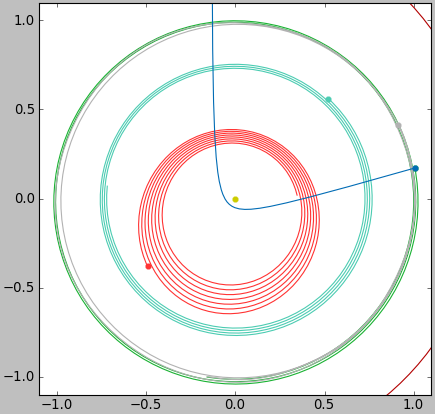
\includegraphics[scale=0.38]{img/bomba/decote.png}
	\label{fig:res_bomba_4}
	}
	\caption{
		Acá vemos la simulación de el proyectil \textit{Bomba Oscura} para una instancia en la que le pega a la tierra,
		con distintas ampliaciones.
		El misil fue disparado desde el punto $<0,30,0>$ AU (aproximadamente) a una velocidad de $<0.00150022,-0.0346204,0>$ AU/día.
		En la última imagen vemos un intento de pegarle a la tierra bastante rebuscado, que paso muy cerca de su objetivo.
		Esto nos muestra que hay muchísimas posibilidades extrañas también de pegarle a la tierra pero que requieren de un cálculo mucho mas fino ya que
		aparecen distancias chicas que vuelven al sistema bastante inestable numericamente.
	}
	\label{ fig:res_bomba }
\end{figure}
